\section{Aufbau}
%bild vom aufbau(das bild muss noch angepasst werden, die neuen baueteile müssen ergänzt werden)
%bild von den ventilen
\begin{figure}
	\centering
	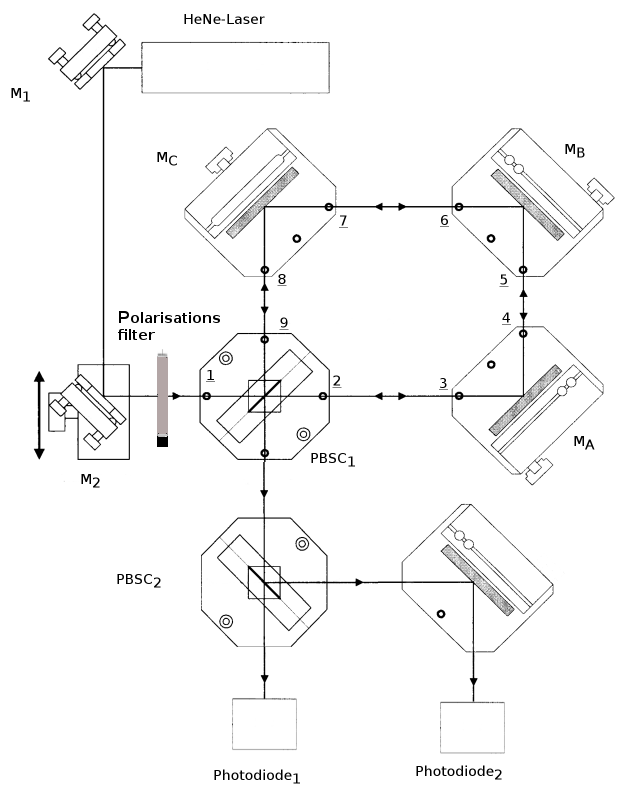
\includegraphics[width=\linewidth-100pt,height=\textheight-100pt,keepaspectratio]{content/Bilder/aufbau1.png}
	\caption{Aufbau des Sagnac Interferometers \cite{V64}.}
	\label{fig:Aufbau}
\end{figure}

\begin{figure}
	\centering
	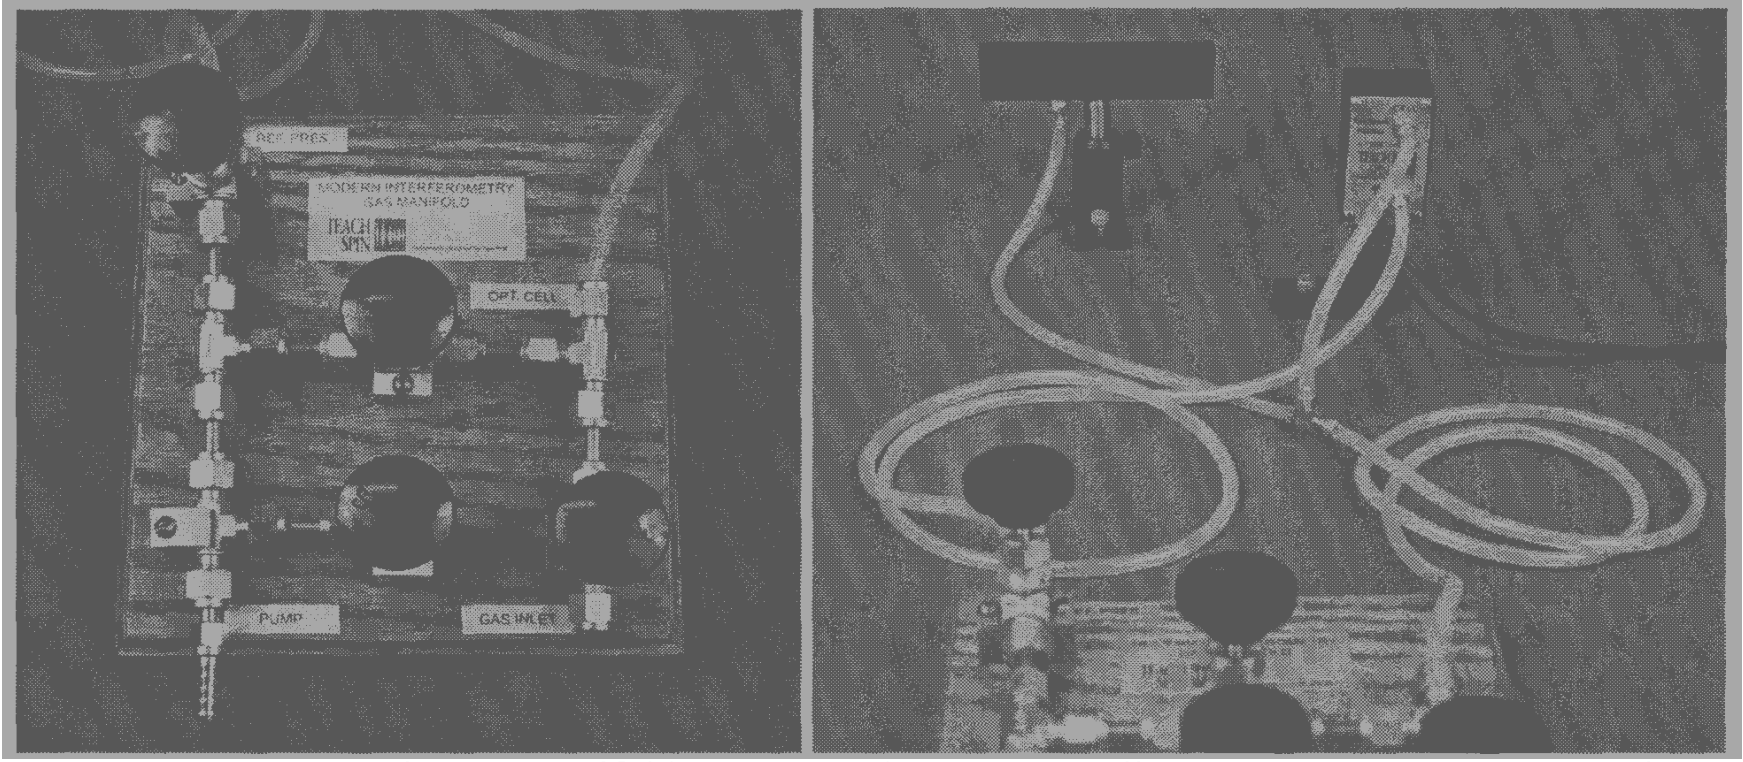
\includegraphics[width=\linewidth-100pt,height=\textheight-100pt,keepaspectratio]{content/Bilder/Gaszellelesskontrast.png}
	\caption{Aufbau der Ventilschaltung der Gaszelle \cite{V64}.}
	\label{fig:Gas}
\end{figure}

Der Aufbau besteht aus einem Sagnac Interferometer gemäß Abb. \ref{fig:Aufbau}. Die Stärke des Sagnac Interferometers ist eine konstruktionsspezifische Stabilität gegenüber äußeren Störeinflüssen wie Vibrationen der Spiegel oder kleinen Luftturbolenzen. ZU Beginn wird der Strahl eines linear polarisierten HeNe Lasers über zwei Lenkspiegel auf einen PBSC gelenkt. Um die Polarisationsrichtung zu variieren wird zusätzlich ein Polarisationsfilter vor den PBSC montiert. In diesem werden die vertikalen und horizontal polarisierten Anteile getrennt, wobei ein Anteil den PBSC grade passiert, während der zweite um $\SI{90}{\degree}$ abgelenkt wird. Beide Strahlen werden gemäß Abb. \ref{fig:Aufbau} über drei Spiegel abgelenkt, sodass die Strahlen diesselben Wege zurücklegen, jedoch mit gegenläufiger Richtung. Um nachher eine Probe in einen einzelnen Strahlengang einzuführen, sind die Lenkspiegel so eingestellt, sodass beide Strahlen räumlich getrennt sind. Während der Durchführung wird entweder eine Gaszelle in einen der Strahlen gesetzt oder es werden zwei drehbare Gläser in die Strahlen gesetzt. Die zugehörige Halterung ist so aufgebaut, dass jeweils ein Glas in einem Strahlengang steht. Die Strahlen werden beim Wiedereintritt in den PBSC wieder zu einem Strahl überlappt. Dieser gelangt in einen zweiten PBSC, welcher um $\SI{45}{\degree}$ gedreht ist. Hinter die Strahlengänge beider resultierender Strahlen ist eine Photodiode gesetzt. Der umgelenkte Strahl läuft dafür nochmals über einen dazwischen montierten Spiegel. Die elektrischen Signale werden gleichermaßen verstärkt und können über ein Oszilloskop betrachtet werden. Zum Schutz vor Störungen durch Luftturbolenzen wird während der Messungen ein Schutz über das Interferometer gesetzt. Die bei der Bestimmung des Brechungsindex von Luft verwendete Gaszelle kann über eine Pumpe und eine Ventilschaltung nach Abb. \ref{fig:Gas} evakuiert und anschließend wieder langsam auf Normaldruck gebracht werden.
%  Zu Beginn wird der Strahl eines HeNe Lasers auf einen über zwei Ausrichtungsspiegel auf einen PBSC gerichtet. Der Strahl ist linear polarisiert und die Quelle ist so gedreht, dass der Vektor des elektromagnetischen Feldes in einem $\SI{45}{\degree}$ Winkel zur Vertikalen Achse steht. Der eintreffende Strahl wird durch einen Strahlteiler in zwei Strahlen, deren Polarisierungen orthogonal zueinander liegen, geteilt. Als Strahlteiler wird ein PBSC verwendet. Zusätzlich gelangt einer der Strahlen gradlinig durch den Strahlteiler, während der zweite Strahl um $\SI{90}{\degree}$ gedreht wird. Beide Strahlen gelangen danach gegenläufig durch die in Abb. \ref{} dargestellte Spiegelkonstruktion aus 3 Spiegeln, welche jeweils im $\SI{45}{\degree}$ Winkel zu den Strahlen aufgestellt wird. Bei genauer Ausrichtung sollen sich beide Strahlen vollständig überlappen, jedoch in entgegengesetzte Richtungen laufen. Am Strahlteiler laufen beide Strahlen wieder zusammen und werden über die vierte Kante wieder zu einem Strahl zusammengeführt. An diesem Punkt liegt jedoch weiterhin keine Phasendifferenz vor. 